\documentclass[a4paper,12pt]{article}
\usepackage{amsmath,amssymb,amsfonts,amsthm}
\usepackage{tikz}
\usepackage [utf8x] {inputenc}
\usepackage [T2A] {fontenc} 
\usepackage[russian]{babel}
\usepackage{cmap} 
\usepackage{ gensymb }
% Так ссылки в PDF будут активны
\usepackage[unicode]{hyperref}
\usepackage{ textcomp }

% вы сможете вставлять картинки командой \includegraphics[width=0.7\textwidth]{ИМЯ ФАЙЛА}
% получается подключать, как минимум, файлы .pdf, .jpg, .png.
\usepackage{graphicx}
% Если вы хотите явно указать поля:
\usepackage[margin=1in]{geometry}
% Или если вы хотите задать поля менее явно (чем больше DIV, тем больше места под текст):
% \usepackage[DIV=10]{typearea}

\usepackage{fancyhdr}

\newcommand{\bbR}{\mathbb R}%теперь вместо длинной команды \mathbb R (множество вещественных чисел) можно писать короткую запись \bbR. Вместо \bbR вы можете вписать любую строчку букв, которая начинается с '\'.
\newcommand{\eps}{\varepsilon}
\newcommand{\bbN}{\mathbb N}
\newcommand{\dif}{\mathrm{d}}

\newtheorem{Def}{Определение}


\pagestyle{fancy}
\makeatletter % сделать "@" "буквой", а не "спецсимволом" - можно использовать "служебные" команды, содержащие @ в названии
\fancyhead[L]{\footnotesize Оптика}%Это будет написано вверху страницы слева
\fancyhead[R]{\footnotesize ФМХФ МФТИ}
\fancyfoot[L]{\footnotesize \@author}%имя автора будет написано внизу страницы слева
\fancyfoot[R]{\thepage}%номер страницы —- внизу справа
\fancyfoot[C]{}%по центру внизу страницы пусто

\renewcommand{\maketitle}{%
	\noindent{\bfseries\scshape\large\@title\ \mdseries\upshape}\par
	\noindent {\large\itshape\@author}
	\vskip 2ex}
\makeatother
\def\dd#1#2{\frac{\partial#1}{\partial#2}}


\title{4.4.1 \\ Амплитудная дифракционная решетка}
\author{Егор Берсенев} 
\date{9 февраля 2017 г.}

\begin{document}
	\maketitle
	\section{Цель работы}
		Знакомство с настройкой и работой гониометра, определение спектральных характеристик амплитудной решетки.
	\section{Оборудование}
	Гониометр Г5, дифракционная решетка, ртутная лампа.
	
	\section{Теоретическое введение}

	Амплитудную решетку можно представить в виде непрозрачного экрана, в котором прорезано большое число $N$ параллельных щелей --- штрихов. Постоянство расстояний между штрихами $d$ и ширина штриха $b$ должны выдерживаться с большой точностью. При наблюдении спектра амплитуда и интенсивность световой волны определяются углом $\varphi$ между нормалью к решетке и направлением дифрагировавших лучей. Будем считать, что амплитуды всех волн одинаковы, т.е. фиксирована амплитуда падающей волны и постоянна площадь всех штрихов. Интенсивность дифрагированного света для углов $\varphi_m$, при которых волны, приходящие в точку наблюдения от всех щелей оказываются в фазе:
	
	\begin{equation}\label{eq:1}
		d\sin\varphi_m = m\lambda
	\end{equation}
	
	Величина $m$ называется порядком спектра.
	
	Угловая дисперсия $D(\lambda)$ характеризует угловое рассеяние между близкими спектральными линиями:
	
	\begin{equation}\label{eq:2}
		D(\lambda) = \frac{\dif\varphi}{\dif\lambda}
	\end{equation}
	
	Для угловой дисперсии решетки получаем:
	
	\begin{equation}\label{eq:3}
		D(\lambda) = \frac{\dif\varphi}{\dif\lambda} = \frac{m}{\sqrt{d^2-m^2\lambda^2}}
	\end{equation}
	
	C увеличением порядка спектра угловая дисперсия будет возрастать. Для малых углов дифракции угловая дисперсия пропорциональна порядку спектра: $D\simeq m/d$.
	
	
	
	
	\section{Ход работы}
		Проведем юстировку гониометра согласно инструкции на установке. Угол $\varphi_0 = 191\degree\, 13'\, 3''$. Проведем измерения спектра $\pm1$ порядка.
		Знак минус у номера спектральной линии обозначает спектр -1 порядка.
		
		
		\begin{table}[h]
			\centering
			\caption{Спектр первого порядка}
			\label{table1}
			\begin{tabular}{|l|l|l|l|l|l|l|}
				\hline
				№ & $\lambda_{th}$  & $\varphi$ & $\varphi-\varphi_0$ & $\sin\left(\varphi-\varphi_0\right)$ & Яркость & Цвет \\ \hline
				1 & 579.1 & $208\degree\, 10'\, 16''$& 0.296 & 0.292 & 10 & желтый  \\ \hline
				2 & 577.0 & $208\degree\, 5'\, 38''$ & 0.295 & 0.290 & 8 & желтый \\ \hline
				3 & 546.1 & $207\degree\, 3'\, 50''$ & 0.277 & 0.273 & 10 & зеленый \\ \hline
				4 & 491.6 & $205\degree\, 25'\, 58''$& 0.248 & 0.246 & 4 & голубой \\ \hline
				5 & 435.8 & $204\degree\, 0'\, 0''$  & 0.223 & 0.221 & 4 & синий \\ \hline
				-1 & 579.1 & $174\degree\, 23'\, 46''$ & -0.294 & 0.289 & 10 & желтый \\ \hline
				-2 & 577.0 & $174\degree\, 26'\, 54''$ & -0.293 & 0.289 & 8 & желтый \\ \hline
				-3 & 546.1 & $175\degree\, 26'\, 42''$ & -0.275 & 0.272 & 10 & зеленый \\ \hline
			\end{tabular}
		\end{table}
	
		Построим график $\sin\Delta\varphi(\lambda)$. По наклона графика оценим шаг решетки.
		
		Для оценки погрешности результат будем считать, что гониометр позволяет измерять углы с точностью не менее, чем 5 угловых секунд. Тогда $$\sigma(\sin\Delta\varphi) \leq \left|\cos\Delta\varphi\right|\sigma(\Delta\varphi) \leq \sigma(\Delta\varphi)$$
		
		Оценим приборную погрешность: $$
		\sigma(\Delta\varphi) \simeq \frac{5}{3600} \simeq 1.3\cdot10^{-3} \ll \sigma_{rand}
		$$
		
		Таким образом, шаг решетки равен $d = 488 \pm 9\, \frac{\text{штрихов}}{\text{мм}}$, что практически в пределах погрешности сходится с фактическим значением в $500\,\frac{\text{штрихов}}{\text{мм}}$.
		
		\begin{figure}[h]
			\caption{График зависимости $\sin\varphi$ от $\lambda$}
			\centering
			\label{pic1}
			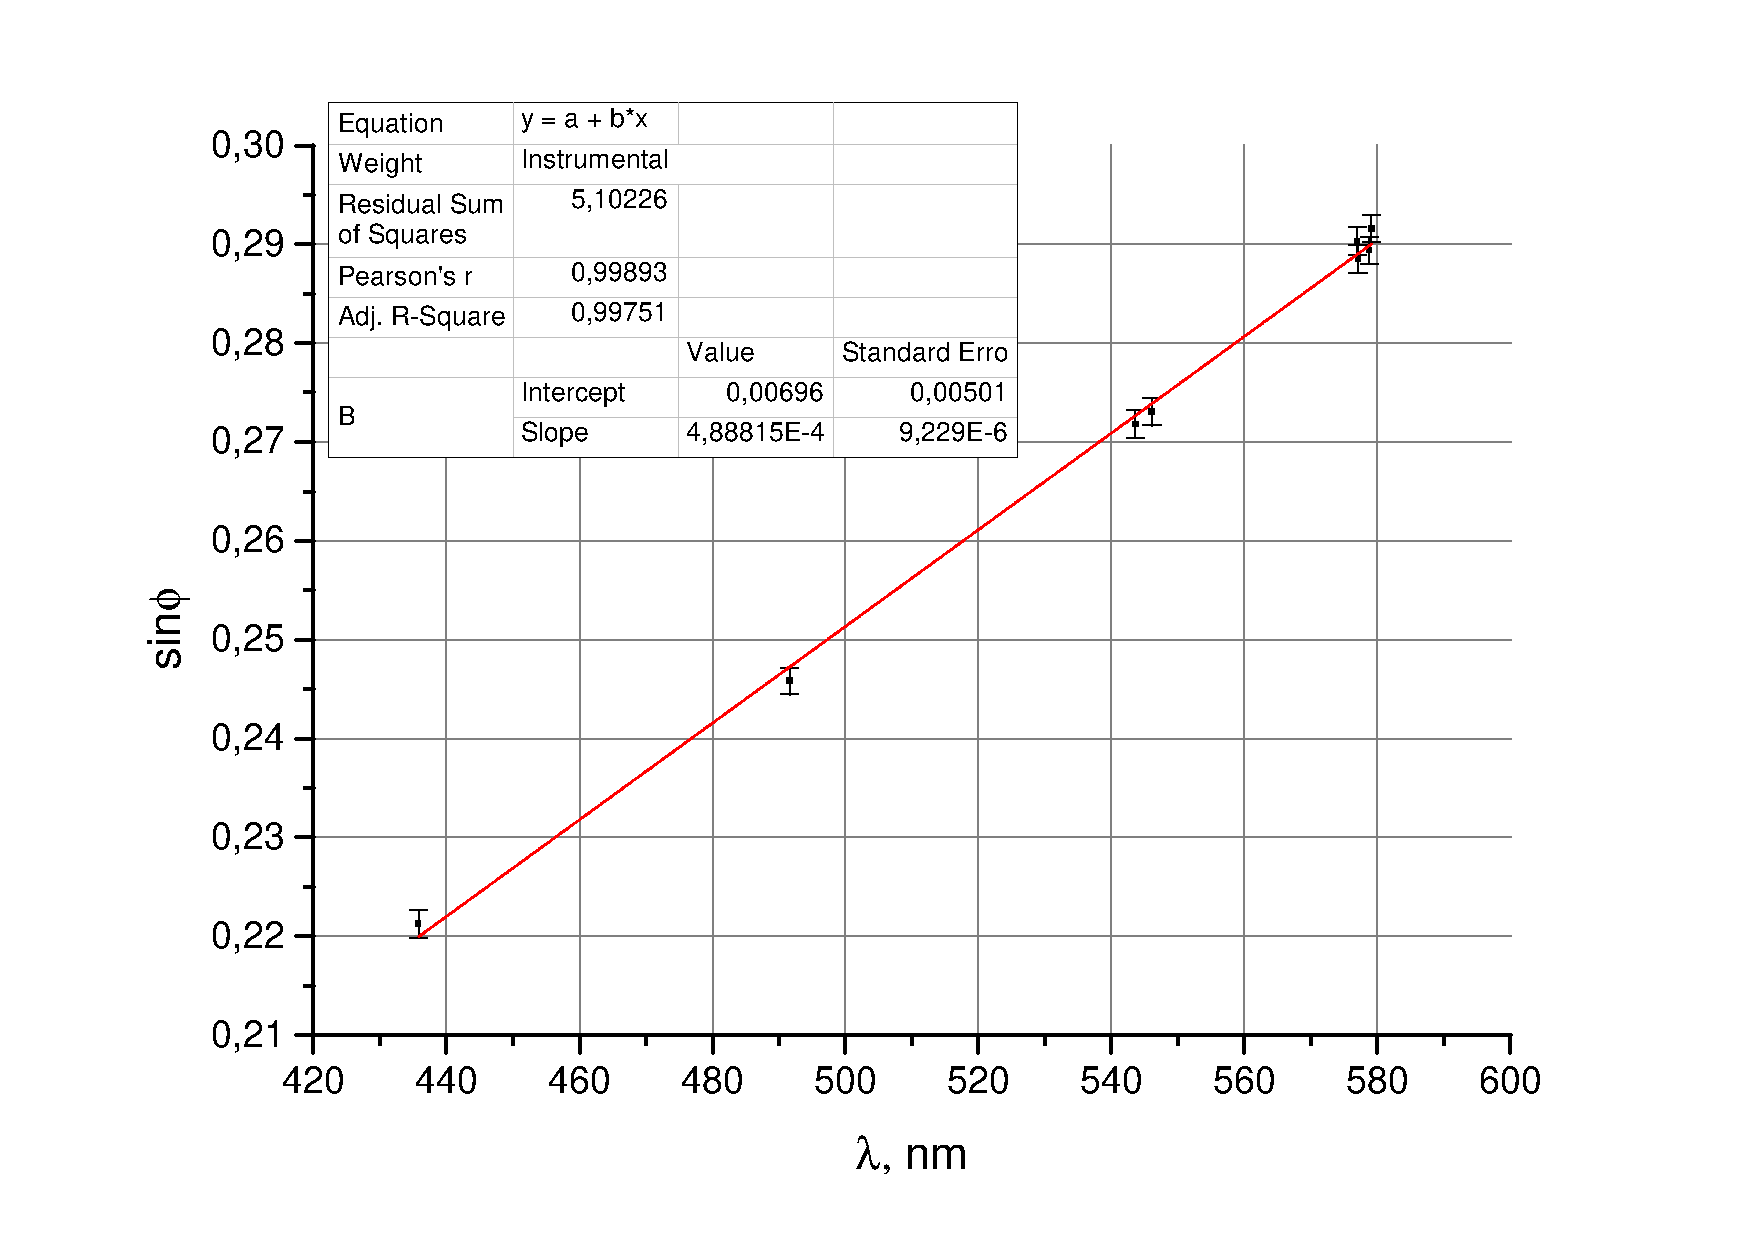
\includegraphics[width = 0.8\linewidth]{graph1}
		\end{figure}

		
		
		Исследуем угловую дисперсию. Для этого выразим $D = \frac{\dif \varphi}{\dif\lambda}$ в угловых секундах на ангстрем полученный для спектральных линий одного порядка и рассчитанную теоретически. Опытные точки на графике обозначим черными квадратами, теоретические красными кругами.
		
		\begin{table}[h]
			\centering
			\caption{Угловая дисперсия для двух желтых линий}
			\label{table2}
			\begin{tabular}{|l|l|l|l|}
				\hline
				№\newline\,  & $\Delta\varphi$, $''$ & $D_{ex}$, $''/\text{\AA}$  & $D_{th}$, $''/$\AA      \\ \hline
				1  & 278  & 13.24  & 10.77 \\ \hline
				-1 & 188  & 8.95   & 10.77 \\ \hline
				-2 & 552  & 26.29  & 25.28 \\ \hline
				-3 & 2400 & 114.29 & 62.09 \\ \hline
			\end{tabular}
		\end{table}
		
		\begin{figure}[h]
			\caption{Угловая дисперсия для спектров разного порядка}
			\centering
			\label{pic2}
			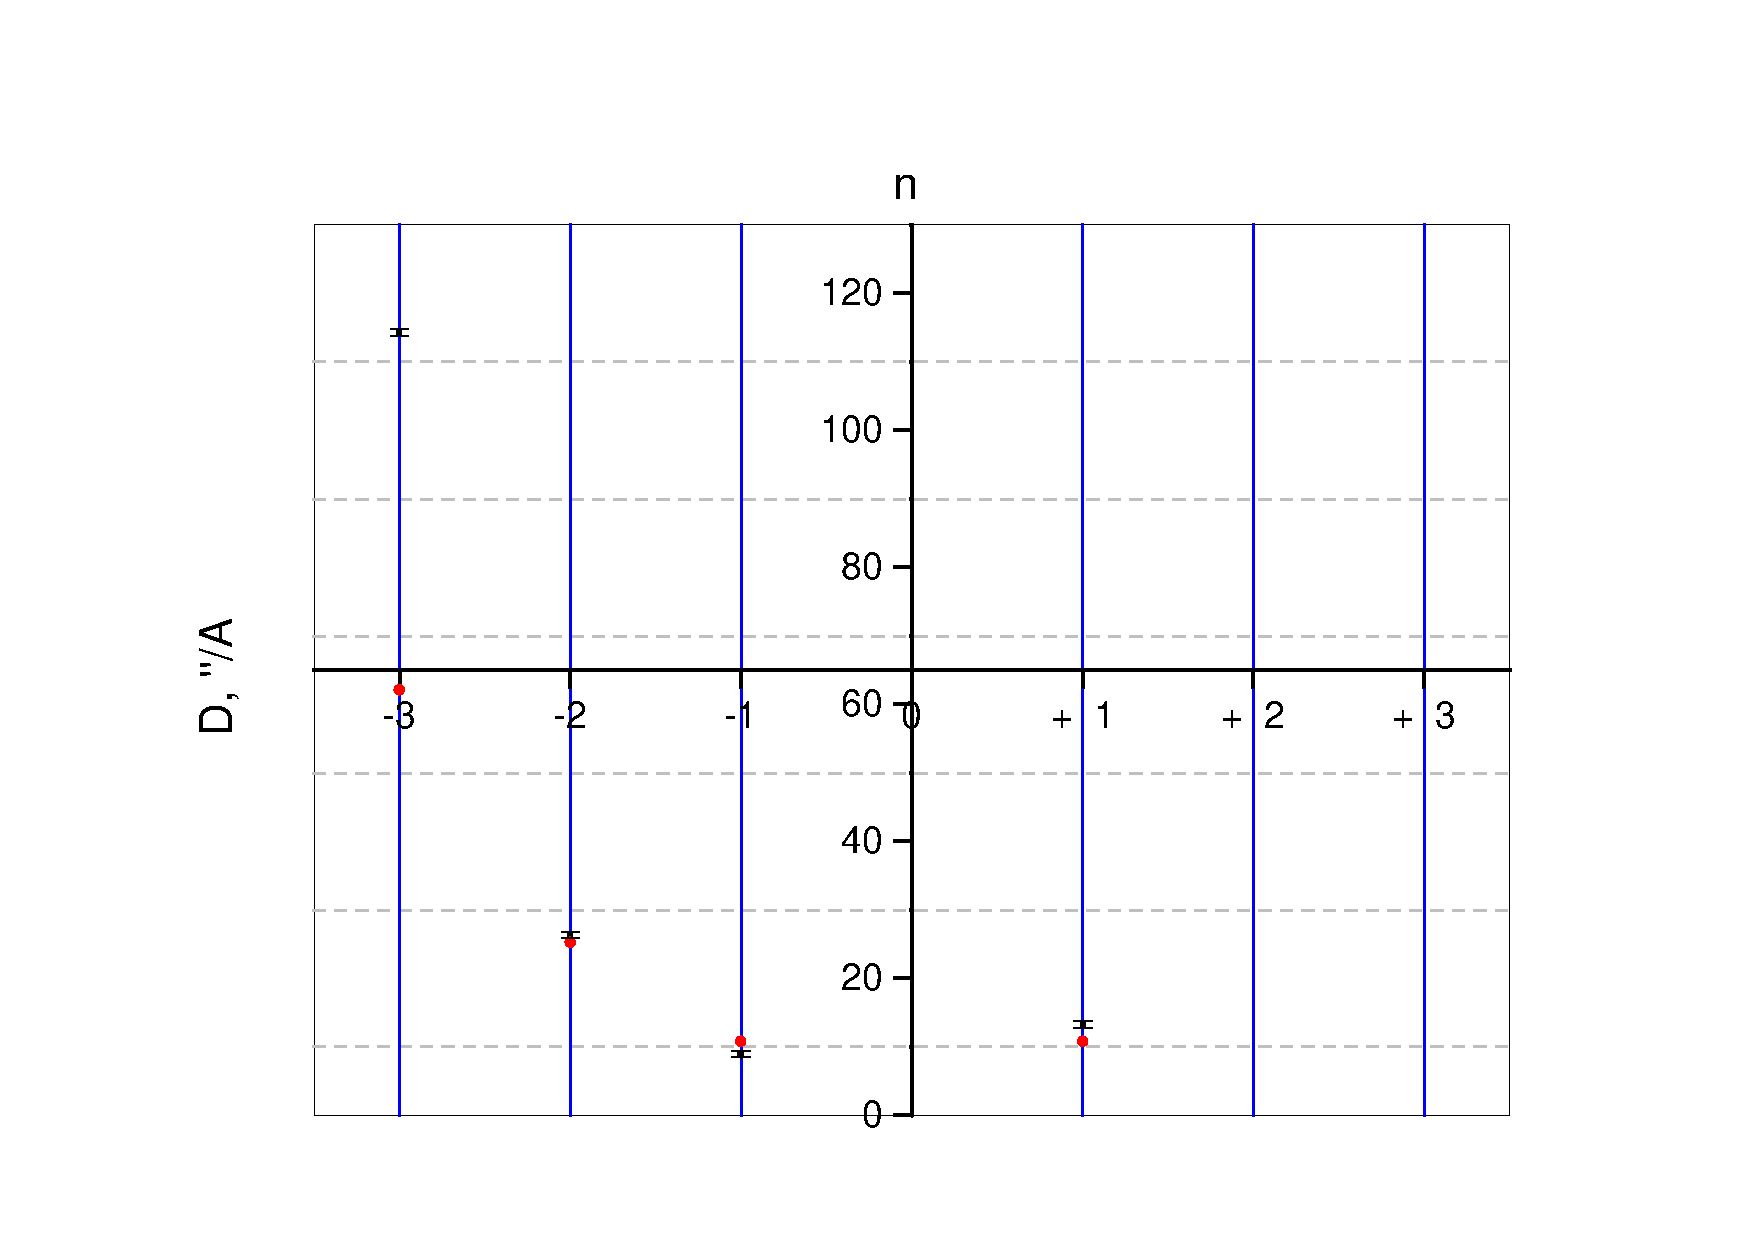
\includegraphics[width = 0.8\linewidth]{graph2}
		\end{figure}
	
	\section{Вывод}
	
		Гониометр, как прибор для точного измерения углов, позволяет работать со спектральными приборами с высокой точностью, и определять неизвестные параметры. Амплитудная дифракционная решетка, как дифракционный прибор позволяет получать достаточно яркие спектры вплоть до третьего порядка.
\end{document}


